\chapter{Results of experiments}

\begin{table}[ht]
\centering
 \begin{tabular}{|p{14cm}|} 
 \hline\hline
 \textbf{Person 1 description:} 1. as a child, i won a national spelling bee. 2. i have been published in the new yorker magazine. 3. i am a gourmet cook. 4. i have perfect pitch. \\
 \hline
 \textbf{Person 2 description:} 1. i am very athletic.  2. i wear contacts. 3. i have brown hair. 4. i love bicycling. 5. i hate carrots. \\
 \hline\hline
 \textbf{Person 1:} hi! i work as a gourmet cook. \\
 \textbf{Person 2:} i do not like carrots. i throw them away.\\ 
 \textbf{Person 1:} really. but, i can sing pitch perfect. \\
 \textbf{Person 2:} i also cook, and i ride my bike to work. \\
 \textbf{Person 1:} great! i had won an award for spelling bee. \\
 \textbf{Person 2:} my contacts can see through what you are trying to sell me. \\
 \textbf{Person 1:} okay but i was published in new yorker once. \\
 \textbf{Person 2:} you better not make any spelling mistakes. \\
 \textbf{Person 1:} i have not. i can cook any word you want me to. \\
 \textbf{Person 2:} what is your ethnicity? i am white, and my hair is brown. \\
 \textbf{Person 1:} i am asian and have no hair. \\
 \textbf{Person 2:} i love hairless asians. \\
 \hline\hline
 \end{tabular}
 \caption{Example of real conversation}
\label{tab:real_conversation}
\end{table}

\begin{table}[ht]
\centering
 \begin{tabular}{|p{7cm}|p{7cm}|} 
 \hline\hline
 \textbf{Person1} & \textbf{Person2} \\
 \hline\hline
 Person's description: 1. as a child, i won a national spelling bee. 2. i have been published in the new yorker magazine. 3. i am a gourmet cook. 4. i have perfect pitch. & Person's description: 1. i am very athletic. 2. i wear contacts. 3. i have brown hair. 4. i love bicycling. 5. i hate carrots. \\
 \hline
 hi, how are you doing today? & that is cool. I am a chef\\ 
 \hline
 i don't like carrots either. I am a gourmet cook.& i am very athletic. i love to play sports \\
 \hline
 i ride my bike to work as well. & that is awesome. i am very athletic, so i love spelling \\
 \hline 
 i have been published in a new yorker magazine & that is cool. i have never heard of it \\
 \hline
 i do not make any spelling mistakes & that is great! \\
 \hline 
 i am from california. my hair is brown & what is your ethnicity? i am asian. \\
 \hline\hline
 \end{tabular}
 \caption{Experiment BART conversation}
\label{tab:bart_conversation}
\end{table}


\begin{table}[ht]
\centering
 \begin{tabular}{|p{14cm}|} 
 \hline\hline
 \textbf{Person 1 description:} as a child, i won a national spelling bee. \# i have been published in the new yorker magazine. \# i am a gourmet cook. \# i have perfect pitch. \\
 \hline
 \textbf{Person 2 description:} i am very athletic. \# i wear contacts. \# i have brown hair. \# i love bicycling. \# i hate carrots. \\
 \hline\hline
 \textbf{Person 1:} (Silence) \\
 \textbf{Person 2:} hello , how are you doing today? \\ 
 \textbf{Person 1:} hi! i work as a gourmet cook \\
 \textbf{Person 2:} what kind of gourmet cook do you cook?\\
 \textbf{Person 1:} i do not like carrots. i throw them away. \\
 \textbf{Person 2:} what kind of carrots do you discard? \\
 \textbf{Person 1:} really. but, i can sing pitch perfect. \\
 \textbf{Person 2:} what kind of music do you sing pitch perfect? \\
 \textbf{Person 1:} i also cook, and i ride my bike to work. \\
 \textbf{Person 2:} that sounds fun! i ride my bike to work as well. \\
 \textbf{Person 1:} great! i had won an award for spelling bee. \\
 \textbf{Person 2:} awesome! what kind of spelling bee did you win? \\
 \hline\hline
 \end{tabular}
 \caption{Experiment BART conversation with specifity, weight = 5}
\label{tab:bart_conversation_idf5}
\end{table}

\begin{table}[ht]
\centering
 \begin{tabular}{|p{7cm}|p{8cm}|} 
 \hline\hline
 \textbf{Person1} & \textbf{Person2} \\
 \hline\hline
 Person description: as a child, i won a national spelling bee. \# i have been published in the new yorker magazine. \# i am a gourmet cook. \# i have perfect pitch. & Person description: i am very athletic. \# i wear contacts. \# i have brown hair. \# i love bicycling. \# i hate carrots. \\
 \hline
 (Silence) & email ...\\ 
 \hline
 hi! i work as a gourmet cook & providing Gourmet Cookery Cookeries produces artisanal artisan sauces costing \$300-\$400 apiece apiece.\\
 \hline
 i do not like carrots. i throw them away. & Carrots contain potassium chloride Sodium sulfoxide oxide oxide coating saltspoon salts iodophenophenols iodidine sulfamate sulfoxin sulfuronium sulphuronicum sulphuranicum sulfuranium sulfenium sulfurous sulfury sulphury sulfioxide sulphurous sulphoric oxide sulphurate sulphur iodassium iodidation sulphuration sulfurate sulfidation sulfurious sulphurized sulphural sulforic acid sulphurus sulfacid sulfural iodoric sulphorus sulfuration iodacid iodidated sulphurred sulphurious sulfitious sulfimony sulf \\
 \hline 
 really. but, i can sing pitch perfect. & sung pitch perfect pitches Perfect?!?!!? !!?! !! !!!!!!!!!!!!!!!!!!!!!!!!!!!!!!!!!!!!!!!!!!!!!!!!!!!!!!!!!!!!!!!! !!!!!!!!!!!!!!! !!!!!!!!!!!!! !!!!! !!!!!!!!!!!!!!! !!!--!--!!!!!!!!~~~~~~~~~~~~~~ !!~~~~!!!!!--~~~~>>>>>>>>~~~~ === ===>>>> ===~~~~== ========== === == === =======>>>>===>>>>==== ===== ======== =====>>>> ===== ==>>>> == ===== ===== ==================== ========= ======>>>> ================= ...\\
 \hline
 i also cook, and i ride my bike to work. & bike Riders Ride Their Bike To Work?!?!!? !!?! !! ... \\
 \hline 
 great! i had won an award for spelling bee. & speech bee Awards Awards Award Award Awards Prize Award Prize Prize Winner Award Winner PrizeWinner AwardWinner Winner WinnerWinnerWinner Prize Winners Award Winners Prize Winning Winner WinningWinner Winning Winners Winners Winning winners Winning finalists Winning losers Winning prizes Winning votes Winning Votes WinningvotesWinner votesWinner Votes WinnersWinner WinnersWinnersWinishersWinessesWinerersWinotersWin finalistsWinner finalistsWin winnersWinner \\
 \hline\hline
 \end{tabular}
 \caption{Experiment BART conversation with specifity, weight = 10}
\label{tab:bart_conversation_idf5}
\end{table}

\begin{table}[ht]
\centering
 \begin{tabular}{|p{14cm}|} 
 \hline\hline
 \textbf{Person 1 description:} as a child, i won a national spelling bee. \# i have been published in the new yorker magazine. \# i am a gourmet cook. \# i have perfect pitch. \\
 \hline
 \textbf{Person 2 description:} i am very athletic. \# i wear contacts. \# i have brown hair. \# i love bicycling. \# i hate carrots. \\
 \hline\hline
 \textbf{Person 1:} (Silence) \\
 \textbf{Person 2:} hi, how are you today? \\ 
 \textbf{Person 1:} hi! i work as a gourmet cook \\
 \textbf{Person 2:} i am a chef. i love to cook \\
 \textbf{Person 1:} i do not like carrots. i throw them away. \\
 \textbf{Person 2:} i do not like carrots. i am not a fan. \\
 \textbf{Person 1:} really. but, i can sing pitch perfect. \\
 \textbf{Person 2:} i am not sure. i do not have a good voice. \\
 \textbf{Person 1:} i also cook, and i ride my bike to work. \\
 \textbf{Person 2:} i have a bike to work. i love it. \\
 \textbf{Person 1:} great! i had won an award for spelling bee. \\
 \textbf{Person 2:} that is great. do you have a favorite color? \\
 \hline\hline
 \end{tabular}
 \caption{Experiment BART conversation with specifity, weight = -5}
\label{tab:bart_conversation_idf5}
\end{table}

\begin{table}[ht]
\centering
 \begin{tabular}{|p{7cm}|p{7cm}|} 
 \hline\hline
 \textbf{Person1} & \textbf{Person2} \\
 \hline\hline
 Person description: as a child, i won a national spelling bee. \# i have been published in the new yorker magazine. \# i am a gourmet cook. \# i have perfect pitch. & Person description: i am very athletic. \# i wear contacts. \# i have brown hair. \# i love bicycling. \# i hate carrots. \\
 \hline
 (Silence) & hi, i am a cook. do you have a job? \\ 
 \hline
 hi! i work as a gourmet cook & i am a cook. i love to cook \\
 \hline
 i do not like carrots. i throw them away. & i do not have a favorite. i am not a fan. \\
 \hline 
 really. but, i can sing pitch perfect. & i am not a very good singer. \\
 \hline
 i also cook, and i ride my bike to work. & i have a bike to work. i love to ride. \\
 \hline 
 great! i had won an award for spelling bee. & that is a good one. i have a lot of fun.. \\
 \hline\hline
 \end{tabular}
 \caption{Experiment BART conversation with specifity, weight = -10}
\label{tab:bart_conversation_idf5}
\end{table}

\begin{table}[ht]
\centering
 \begin{tabular}{|p{7cm}|p{7cm}|} 
 \hline\hline
 \textbf{Person1} & \textbf{Person2} \\
 \hline\hline
 Person description: as a child, i won a national spelling bee. \# i have been published in the new yorker magazine. \# i am a gourmet cook. \# i have perfect pitch. & Person description: i am very athletic. \# i wear contacts. \# i have brown hair. \# i love bicycling. \# i hate carrots. \\
 \hline
 (Silence) & hey! how are you today? \\ 
 \hline
 hi! i work as a gourmet cook & i was just about to go to a gourmet cook shop. \\
 \hline
 i do not like carrots. i throw them away. & i am a chef for carrots.\\
 \hline 
 really. but, i can sing pitch perfect. & i love the chorus. \\
 \hline
 i also cook, and i ride my bike to work. & i love riding my bike. \\
 \hline 
 great! i had won an award for spelling bee. & that is awesome. i am sure! \\
 \hline\hline
 \end{tabular}
 \caption{Experiment BART with GPT-2 7:3}
\label{tab:bart_conversation_gpt2}
\end{table}

\begin{table}[ht]
\centering
 \begin{tabular}{|p{14cm}|} 
 \hline\hline
 \textbf{Person 1 description:} 1. my mom is my best friend. 2. i have four sisters. 3. i believe that mermaids are real. 4. i love iced tea \\
 \hline
 \textbf{Person 2 description:} 1. i got married last year. 2. i live on a boat. 3. my hair is colored purple. 4. i have my own salon. 5. i am a hair stylist \\
 \hline\hline
 \textbf{Person1:} hello, how are you doing? \\
 \textbf{Person2:} hi there, i am doing great thanks. where are you from?\\ 
 \textbf{Person1:} i am from socal, yourself? \\
 \textbf{Person2:} seattle. i have a houseboat here. i like socal weather though\\
 \textbf{Person1:} that is awesome. the ocean is incredible! i totally believe that mermaids are out in the sea \\
 \textbf{Person2:} lol definitely! i just dyed my hair mermaid purple from free samples at my salon \\
 \textbf{Person1:} that is epic! me and my four sisters would totally do the same thing!! \\
 \textbf{Person2:} oh yeah, i am a stylist here and i have lots of clients doing fantasy colors \\
 \textbf{Person1:} oh nice ! my mom went to beauty school too \\
 \textbf{Person2:} oh awesome! well you guys are all set! are you married? \\
 \textbf{Person1:} she still braids my hair and we chit chat because she is literally my best friend \\
 \textbf{Person2:} awww, that is precious. i feel the same way about my mom \\
 \hline\hline
 \end{tabular}
 \caption{Example 2 of real conversation.}
\label{tab:real_conversation_2}
\end{table}

\begin{table}[ht]
\centering
 \begin{tabular}{|p{14cm}|} 
 \hline\hline
 \textbf{Person 1 description:} 1. my mom is my best friend. 2. i have four sisters. 3. i believe that mermaids are real. 4. i love iced tea \\
 \hline
 \textbf{Person 2 description:} 1. i got married last year. 2. i live on a boat. 3. my hair is colored purple. 4. i have my own salon. 5. i am a hair stylist \\
 \hline\hline
 \textbf{Person1:} i love iced tea. i love it. \\
 \textbf{Person2:} i am doing well. how are you? \\ 
 \textbf{Person1:} i am from california, you? \\
 \textbf{Person2:} i am from california. i live on a boat.\\
 \textbf{Person1:} sounds like a great place to live. \\
 \textbf{Person2:} sounds like a lot of fun. do you have any hobbies? \\
 \textbf{Person1:} sounds like a good idea. i am a hair stylist myself. \\
 \textbf{Person2:} sounds like a lot of fun! do you have any siblings? \\
 \textbf{Person1:} sounds like a lot of fun! i like fantasy colors. \\
 \textbf{Person2:} sounds like a great job! i am so glad you have a mom! \\
 \hline\hline
 \end{tabular}
 \caption{Experiment BART with tf-idf of SST positive.}
\label{tab:bart_tfidf_sst_pos}
\end{table}

\begin{table}[ht]
\centering
 \begin{tabular}{|p{14cm}|} 
 \hline\hline
 \textbf{Person 1 description:} as a child, i won a national spelling bee. \# i have been published in the new yorker magazine. \# i am a gourmet cook. \# i have perfect pitch. \\
 \hline
 \textbf{Person 2 description:} i am very athletic. \# i wear contacts. \# i have brown hair. \# i love bicycling. \# i hate carrots. \\
 \hline\hline
 \textbf{Person1:} (Silence) \\
 \textbf{Person2:} hi there, how shall we get on?  \\ 
 \textbf{Person1:} i love carrots. i know how you feel. \\
 \textbf{Person2:} i do not know what to do, My lord. \\
 \textbf{Person1:} i am not a great singer. \\
 \textbf{Person2:} i ride to work \\
 \textbf{Person1:} that is the same. \\
 \textbf{Person2:} i am not heard of that. \\
 \textbf{Person1:} i am not very good writer, but I am very good poet. \\
 \textbf{Person2:} i am not a spelling student. But i have a question for you. \\
 \textbf{Person1:} i am not a cook, I am a gourmet cook \\
 \textbf{Person2:} i am not a fool. But I am a man of color  \\
 \hline\hline
 \end{tabular}
 \caption{Experiment BART and GPT2 with Shakespear style}
\label{tab:poetic_shakespear}
\end{table}

\chapter{Luong attention} \label{luong_attn_appendix}

Information in this chapter is taken from \cite{luong2015effective}.
\begin{figure}[hbt]
  \centering
  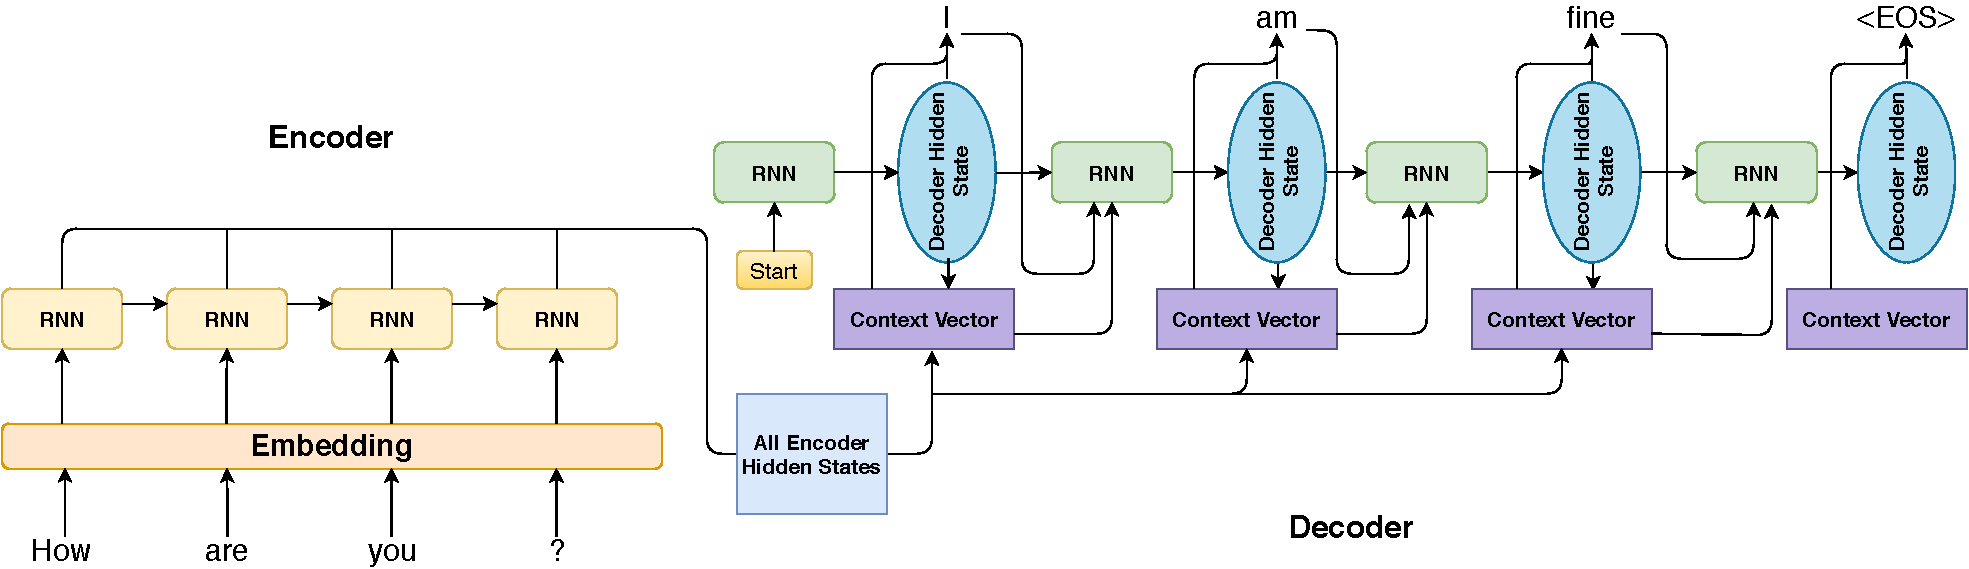
\includegraphics[width=1\textwidth]{figures/luong_decoder.pdf}
  \caption{Luong decoder architecture.}
  \label{luong}
\end{figure}

Luong attention model is classified into 2 categories, \textit{global} and \textit{local}. Common to these types of model is the fact that at each time step \textit{t} in the decoding phase previous hidden state is taken as input to derive a context vector $\mathbf{c_t}$, that captures relevant information to predict the current target word $y_t$. This categories differ only if ``attention'' is placed on all source positions or on a few source positions.

The simple concatenation layer combines the information from vectors $h_t$ and $c_t$ to produce an attentional hidden state (Equation \ref{eq:hs}).
\begin{equation} \label{eq:hs}
\mathbf{\widetilde{h_t}} = tanh(\mathbf{W_c}[\mathbf{c_t};\mathbf{h_t}])
\end{equation}

The attention vector $\mathbf{\widetilde{h_t}}$ then passed through the softmax layer to produce the predictive distribution (Equation \ref{eq:sfm}).
\begin{equation} \label{eq:sfm}
p(y_t|y_{<t},x) = softmax(\mathbf{W_s}\mathbf{\widetilde{h_t}})
\end{equation}

\subsubsection{Global Attention}
An alignment vector $a_t$ (size of $a_t$ is equal to the number of time steps on the source side) is derived by comparing the current target hidden state $\mathbf{h_t}$ with each source hidden state $\mathbf{\bar{h}_s}$ (Equation \ref{eq:av}).
\begin{equation} \label{eq:av}
a_t(s) = align(\mathbf{h_t}, \mathbf{\bar{h}_s}) = \frac{exp(score(\mathbf{h_t}, \mathbf{\bar{h}_s}))}{\sum_{s'} exp(score(\mathbf{h_t}, \mathbf{\bar{h}_s}))}
\end{equation}

There are three types of the score function (the score function is referred as a content-based function) (Equation \ref{eq:sf}).
\begin{equation}\label{eq:sf}
score(\mathbf{h_t}, \mathbf{\bar{h}_s}) = \begin{cases} \mathbf{h_t}^\intercal \mathbf{\bar{h}_s}, & \mbox{dot} \\ \mathbf{h_t}^\intercal \mathbf{W_a} \mathbf{\bar{h}_s}, & \mbox{general} \\ \mathbf{v_a}^\intercal tanh(\mathbf{W_a} [\mathbf{h_t}; \mathbf{\bar{h}_s}]), & \mbox{concat} \end{cases}
\end{equation}

In location-based function the alignment scores are computed from solely the target hidden state $\mathbf{h_t}$ (Equation \ref{eq:sfm_as}).
\begin{equation} \label{eq:sfm_as}
a_t = softmax(\mathbf{W_a}\mathbf{h_t})
\end{equation}

The context vector $\mathbf{c_t}$ is computed as the weighted average over all the source hidden state, where alignment vector represents weights.

\subsubsection{Local Attention}
Global attention is expensive, because it has to attend to all words on the source side for each target word. Local attention chooses to focus only on a small subset of the source positions per target word.

The local alignment vector $a_t$ in this category of attention is fixed-dimensional, because of it there are 2 variants of the model, \textit{monotonic} (Equation \ref{eq:monotonic}) and \textit{predictive} (Equation \ref{eq:predictive}).

\begin{equation} \label{eq:monotonic}
p_t = t
\end{equation}

\begin{equation} \label{eq:predictive}
p_t = S \cdot sigmoid(\mathbf{v_p}^\intercal tanh(\mathbf{W_p} \mathbf{h_t}))
\end{equation}

In monotonic alignment the source and target sequences are roughly monotonically aligned. In predictive alignment the model learns to predict the alignment position, where $\mathbf{W_p}$ and $\mathbf{v_p}$ are the learned model parameters.

Gaussian distribution centered in $p_t$ is used to favor alignment points near $p_t$ (Equation \ref{eq:align_gaus}).
\begin{equation} \label{eq:align_gaus}
a_t(s) = align(\mathbf{h_t}, \mathbf{\bar{h}_s}) exp(-\frac{(s-p_t)^2}{2\sigma^2})
\end{equation}

